\documentclass{article}
\title{Relazione 1 : Errori di computazione delle variabili Floating Point}
\author{Antonio Michele Miti}

\usepackage{amsmath}
\usepackage{amsfonts}
\usepackage[utf8]{inputenc}
\usepackage[italian]{babel}
\usepackage{listings}
\usepackage{textcomp}
\usepackage{graphicx}
\usepackage{subfigure}
\usepackage{rotating}
\usepackage{caption}
\usepackage{latexsym}
\usepackage{epstopdf}
\usepackage{eepic,epic,eepicemu}
\usepackage{color}
\pagestyle{headings}
\definecolor{listinggray}{gray}{0.9}
\definecolor{lbcolor}{rgb}{0.95,0.95,0.95}
\lstset{
	backgroundcolor=\color{lbcolor},
	rulecolor=,
	language=C++,
        basicstyle=\scriptsize,
        upquote=true,
        aboveskip={1.5\baselineskip},
        columns=fixed,
        showstringspaces=false,
        extendedchars=true,
        breaklines=true,
        prebreak = \raisebox{0ex}[0ex][0ex]{\ensuremath{\hookleftarrow}},
        frame=single,
        showtabs=false,
        showspaces=false,
        showstringspaces=false,
        identifierstyle=\ttfamily,
        keywordstyle=\color[rgb]{0,0,1},
        commentstyle=\color[rgb]{0.133,0.545,0.133},
        stringstyle=\color[rgb]{0.627,0.126,0.941},
}
\addtolength{\hoffset}{-1.25cm}
\addtolength{\voffset}{-1.80cm}
\addtolength{\textwidth}{1cm}
\addtolength{\textheight}{3.80cm}
\newtheorem{legge}{Definizione}

\begin{document}
\maketitle
\begin{abstract}
In questo articolo viene trattato l'errore dovuto all'allocazione è alla somma tra variabili float a precisione finita.
In particolare viene studiato l'imprecisione sul risultato che presenta il calcolo di una serie al calcolatore.
\end{abstract}

%\tableofcontents

\section{Introduzione}
\subsection{Rappresentazione in virgola mobile di numeri reali}
\paragraph{Numerazione in base qualsiasi}

Un qualsiasi numero reale $x\in \mathbb{R}$ , previa scelta di un numero pari $b \in \mathbb{N}$ detto base della notazione , può essere rappresentato nella forma:
	\begin{equation}
	x= M \times \beta^{e}
	\end{equation}
$M$ è detta mantissa del numero ed $e$ è detto esponente.

La mantissa è una stringa di p cifre ( p è detta precisione) del tipo:
$$ d_{0} \, , \, d_{1} d_{2} \ldots d_{p-1} \qquad , (0 \leq d_{i} < b)$$
tale che $d_{0} \, , \, d_{1} d_{2} \ldots d_{p-1} \times \beta^{e}$ rappresenta il numero reale
	\begin{equation}
	\pm(d_{0} + d_{1}\beta ^{-1} + \ldots + d_{p-1}\beta ^{-(p-1)})\beta^{e} 
	\end{equation}

idealmente è possibile immaginare un numero float (quindi una mantissa, una stringa di $d_{j} \in \lbrace 0,1,2,\ldots,b-1 \rbrace \subset N \, \forall j $ )a precisione infinita che rappresenti tutti i possibili numeri reali elementi di $\mathbb{R}$:
	\begin{equation}
	\beta^{e}\sum_{k=0}^{\infty}d_{k}b^{-k}
	\end{equation}

Osservazione: qui si sta parlando di numeri e di rappresentazione di numeri, queste idee pur essendo concettualmente separate, vengono praticamente considerate la stessa cosa.

I numeri due, tre, $\pi$ sono elementi del insieme dei numeri reali definito dalla sua struttura di \emph{campo} sono oggetti assoluti.
I simboli 2 e 3 (in base dieci) oppure 010 e 011 ( intero in binario) non sono altro che la rappresentazione degli oggetti fondamentali "due" e "tre" elementi dell'insieme $\mathbb{R}$. 

Il punto di tutto questo discorso è che quando si afferma che l'equazione [1] rappresenta il numero [3], in realtà si sta affermando che [1] e [3] sono rappresentazioni equivalenti dello stesso elemento del campo $\mathbb{R}$.
l'eq [3] può essere intesa solo come rappresentazione in base 10 di quel numero, ovvero la cosiddetta rappresentazione decimale che nella definizione istintiva dell'aritmetica, definisce il numero stesso.

\paragraph{Numerazione in base 2}

In ambito elettronico (quindi anche nell'ambito computazionale) l'unica base possibile per la rappresentazione di un numero è la base 2.
Lo standard IEEE 754 è un insieme di convenzioni, utilizzate nei computer attuali, per la rappresentazione, l'aritmetica e l'arrotondamendo dei numeri in virgola mobile in base 2 nei calcolatori.

Esistono in questo standard tre formati per i numeri in virgola mobile: a precisione singola o \emph{float} (32 bit), precisione doppia o \emph{double} (64 bit) e precisione doppia estesa o \emph{long double}(80 bit).

Un numero in virgola mobile viene quindi rappresentato da parole di 32, 64 o 80 bit divisi in tre
parti:
\begin{itemize}
	\item[-]	un bit di segno $s$;
	\item[-]	un campo di esponente $E$, contenente la cifra dell'esponente in forma intera, formato da $e$ bit;
	\item[-]	un campo di mantissa $M$ formato da $m$ bit;
\end{itemize}
in questo ordine. 

I bit di una parola di n bit sono indicizzati in modo decrescente con numeri interi da 0 a n-1. In un numero, in questo standard, l'importanza del bit decresce col suo indice.

\begin{lstlisting}[frame=single]
 1    e               m            lunghezza in bit
+-+--------+-----------------------+
|S| Esp.   | Mantissa              |
+-+--------+-----------------------+
n-1                                0 indice dei bit
\end{lstlisting}

Il corrispettivo numero in base $10$ può quindi essere calcolato come:
	\begin{equation}
	(-1)^{s} \times 2^{e} \times m \qquad .
	\end{equation}

Il numero $m$ di bit della mantissa corrisponde alla precisione della rappresentazione floating point.
L'esponente, essendo rappresentato come una variabile intera, può assumere $2^{e}$ possibili valori, al primo e all'ultimo di questi lo standard IEEE associa delle funzioni speciali (come ad esempio la rapprasentazione dello zero, del nan o del infinito).

\subsection{unicità della rappresentazione}
Le rappresentazioni in virgola mobile non sono necessariamente uniche, ad esempio $0.01 \times 10^{1}$ e $1.00 \times 10^{-1}$ rappresentano entrambi lo stesso numero.

Si può imporre una notazione in cui la cifra più significativa, $d_{0}$ nella notazione delle formula (2), sia sempre diversa da zero, Tale notazione è detta normalizzata.

Richiedere che la rappresentazione sia normalizzata risolve questa ambiguità della notazione, l'unico problema è che lo zero non è un numero di per se normalizzabile.
Lo standard IEEE 754 aggira questo problema associandogli il numero $1.0 \times \beta ^{e_{min}-1}$


\subsection{Problemi della rappresentazione floating point}

\paragraph{Troncamento della mantissa}

Idealmente la mantissa di un numero reale in base 2 è costituita da un vettore  $v_{k}$ formato da infiniti elementi tali che:
$$M= \sum_{k=0}^{\infty}v_{k}(\dfrac{1}{2})^{k}$$
Nel caso però che si abbiano a disposizione solo N bit per rappresentare la mantissa si definisce la mantissa troncata del numero:
$$\bar{M}=\sum_{k=0}^{p}v_{k}(\frac{1}{2})^{k} \qquad .$$

Che errore porta l'approssimazione $M\simeq\bar{M}$ ?
ricordando la convergenza della serie geometrica di ragione $\mid x \mid <1$ vale che
$$
\sum_{k=0}^{\infty}x^{k} =\lim_{n \rightarrow \infty}\sum_{k=0}^{n}x^{k}=\lim_{n \rightarrow \infty}\frac{1-x^{n+1}}{1-x}=\frac{1}{1-x}
$$
da cui:
	\begin{equation}
\textrm{sup}(M-\bar{M})= \sum_{k=p+1}^{\infty}\frac{1}{2}^{k} =\frac{1}{2}^{p+1}\sum_{k=0}^{\infty}\frac{1}{2}^{k}= \frac{1}{2}^{p+1}\frac{1}{1-\frac{1}{2}} =\frac{1}{2}^{p}
	\end{equation}
viene preso l'estremo superiore in modo da prendere in considerazione il caso peggiore  in cui tutti i $v_{k}$ con $k>N$ sono 1; ovviamente se il numero è composizione lineare di potenze di due può essere rappresentato esattamente da una stringa finita di cifre binarie.

Questo dimostra che il resto di un troncamento alla cifra p di un numero float e dell'ordine di grandezza della cifra p per cui l'ultimo bit significativo è necessariamente affetto da un errore.

Questa errore dipende ovviamente dal numero di bit che la variabile (float, double, long double) utilizza per rappresentare la mantissa ma anche dal numero in se (se è più grande della più grande mantissa rappresentabile richiederà di scalare la virgola e quindi di considerare uno zero davanti come cifra significativa).

In sostanza la precisione determina il numero massimo di cifre significative che vengono memorizzate, l'errore che ne risulta non è assoluto ma percentuale.

\paragraph{Assorbimento nelle Somme}

Il principale problema dell'aritmetica floating point risiede nel errore da troncamento, quest'errore è conseguenza diretta dell'algoritmo del calcolo aritmetico della somma.

L'algoritmo per le addizioni e le sottrazioni è il seguente:
si supponga di sommare due variabili float a precisione p; siano le mantisse $s_{1}$ , $s_{2}$ e $ e_{1} , e_{2}$ i relativi esponenti, tali che $ e_{1} - e_{2} = q$.
\begin{itemize}
	\item[-]	(1)	\emph{shift}: per fare in modo che le due mantisse siano confrontate si "denormalizza"  il numero più piccolo ponendo $ e_{2} = e_{1}$ e spostando la virgola della mantissa $s_{2}$ di q posti verso sinistra.
Siccome il numero è a precisione finita le ultime q cifre significative verranno perse.
	\item[-]	(2) \emph{addizione}: le 2 mantisse possono essere ora sommate bit a bit a dare la mantissa del risultato dell'opeazione.
	\item[-]	(3) \emph{arrotondamento}: il risultato viene quindi troncato a p cifre significative e normalizzato se necessario.
\end{itemize}

Da questo risulta evidente come sia in realtà l'operazione di shift la causa dell'errore, l'arrotondamento è in realtà la normale allocazione di una cifra come variabile float.

Il caso limite di questo effetto è l'azzeramento del minore dei 2 addendi, questo avviene quando si cerca di sommare 2 numeri tali che $ e_{2} - e_{1} \geq p$ per cui lo shift trasla la prima cifra significativa fuori dai bit consentito dalla precisione della variabile.

\section{Caso di Studio}

Alla luce dei problemi appena visti prima sorge il problema di stabilire come calcolare una serie del tipo:
	\begin{equation}
\sum_{n=1}^{\infty}\frac{1}{n}^{2}= \frac{\pi^{2}}{6}
	\end{equation}
con il minore errore possibile.

La questione è di grande importanza dato che la maggior parte dei metodi numerici si basa sul calcolo della convergenza di una serie.

In una serie convergente il termine n-simo della sommatoria tende a 0 al crescere di n per cui man mano che aumentano le iterazioni vengono calcolate addizioni con numeri sempre più piccoli, questo porta ad un errore di troncamento molto grande.

L'unico modo per ammortizare questo errore è quello di raccogliere i termini della sommatoria in modo da sommare sempre valori di ordine di grandezza simile.


\section{Metodologia}

\subsection{Determinare errore di allocazione}
Il fatto che la rappresentazione in binario sia limitata dalla precisione ad un numero finito di bit e il conseguente troncamento della mantissa si ripercuote sulla cifra che effettivamente viene allocata.
Il semplice passaggio di allocare una determinata cifra come una variabile in virgola mobile nella memomoria porta con se degli errori.

La cosa si può mostrare in modo diretto creando un programma \emph{C++} che si limita a salvare il valore di pigreco, dato esatto fino alla 50-sima cifra decimale, come variabile floating point in diverse precisioni. 
Facendo poi stampare questo valore si nota subito che il valore ottenuto coincide con quello che si intendeva utilizzare solo fino ad una certa cifra significativa.

Allo stesso modo si può mostrare un trabocchetto insito nella rappresentazione in basi diverse, un numero che ha un numero finito di cifre decimali in una base non è detto che lo abbia anche in tutte le altre.
Allocando il numero $0.1$ in una variabile float si rende evidente questo fatto. Il valore della variabile stampato dal computer sarà molto vicino al valore originale ma presenta comunque un errore in quanto non è composizione lineare di potenze di $\frac{1}{2}$.

Un altro metodo per stimare l'errore nel allocazione di un numero floating point sfrutta il fenomeno di assorbimento delle somme, in sostanza si cerca per quale valore di $n$ il numero $1/2^{n}$ (termine n-simo della soerie) viene assorbito nella somma con il valore $1$ allocato come float.

Siccome la mantissa di 1 in binario è un 1 seguito da $(p-1)$ zeri sommargli il numero $1/2^{n}$ equivale a sostituire con un 1 l'n-simo zero della stringa, se n supera la precisione p il numero viene assorbito.

Questo si può implementare in \emph{C++} come segue:
\begin{lstlisting}[frame=single]
	float somma=0;
	float precisione= 1.f;
	int bit = 0;  
	while(somma!=1)
    {
		bit++1;
		somma=1.f+precisione;
		precisione=precisione/2;
    }
	bit = bit -1 ;
	errorerelativo = (precisione*4)/1;
\end{lstlisting}

Da questo si ottiene la dimensione in bit della mantissa della variabile floating point usata (in questo esempio è il "float") e la più piccola quantità che la somma numero $1$ non assorbe, da cui si può stimare l'errore percentuale.

\subsection{Calcolo della Serie}

Il modo più istintivo per implementare un programma \emph{C++} che calcoli una serie è con un ciclo for del tipo:

\begin{lstlisting}[frame=single]
float sum1=0;
	for(unsigned int i=1 ; i<=N ;i=i+1)
		{
		float a= 1/((double)i*i);
		sum1= sum1+a;
		}
\end{lstlisting}

il problema di questo programma è che quando i termini n-simi della somma $a_{n} = 1/n^{2}$ sono più piccoli di $2^{-p}$ volte la somma parziale, vengono automaticamente assorbiti.
Tutti i termini $a_{n}$ tali che:
\begin{displaymath}
\frac{1}{n^{2}}\leq 2^{-p}\rightarrow n\geq 2^{p/2}
\end{displaymath}
nel confronto con l'unità, primo termine della serie, verranno azzerati dallo shift.

Il calcolo della somma risulta quindi necessariamente troncato al termine $ n = 2^{p/2} $, è evidente che l'efficienza del'algortimo è legata alla precisione della variabile usata, ma in ogni caso non è possibile far tendere la sommatoria all'infinto arbitrariamente.

Come detto prima la soluzione migliore per diminuire l'errore su una sommatoria è addizionare prima i termini della serie dello stesso ordine di grandezza.
Considerando che la serie è convergente un modo semplice per farlo è cominciare a sommare i termini al contrario, dal più piccolo al più grande, in questo modo la somma parziale è sempre di ordine di grandezza simile ai termini da addizionare e l'errore da assorbimento viene ridotto.
Si realizza quindi la funzione \emph{C++} :

\begin{lstlisting}[frame=single]
float rovescio(long int N)
	{
	float sum2=0;
	for(long int j=0 ; j<=N-1 ;j=j+1)
		{
		long int i= (N-j);
		float a= 1/((float)i*i);
		sum2= sum2+a;
		}
	return(sum2);
	}
\end{lstlisting}

\section{Risultati}

\subsection{Precisione delle Variabili}

Eseguendo il programma mostrato nel paragrafo 3.2 si ottengono i seguenti valori:
\begin{center}
\begin{tabular}{|c|c|c|}
\hline
& \\tipo variabile & bit mantissa & imprecisione relativa \\
\hline
& \\float & 24 & $\sim 10^{-7} \div$ \\
\hline
& \\double & 53 & $\sim 10^{-16} \div$ \\
\hline
& \\long double & 64 & $\sim 10^{-19} \div$ \\
\hline
\end{tabular}
\end{center}

questi valori si possono verificare in modo diretto salvando $\pi$ esatto fino alla $50°$ cifra decimale e quindi stampando il numero effettivamente contenuto nella variabile in cui è stato salvato.
In questo modo si ottiene:

\begin{lstlisting}[frame=single]
          |       !  |         |         |         |         |
 float=   3.14159274101257324218750000000000000000000000000000
 double=  3.14159265358979311599796346854418516159057617187500
 longDo=  3.14159265358979323851280895940618620443274267017841
 vero=    3.14159265358979323846264338327950288419716939937510
           |         |     !  !|         |         |         |
\end{lstlisting}

Con il punto esclamatico è segnata la prima cifra errata, come si può vedere l'errore coincide con quanto ottenuto con il programma precedente.

In modo simile si può anche dimostrare la non corretta rappresentabilità di alcuni numeri che in base 10 sarebbero razionali, per esempio il valore $0,1$:

\begin{lstlisting}[frame=single]
           |         |         |         |
 float=   0.100000001490116119384765625000 
 double=  0.100000000000000005551115123125 
 longDo=  0.100000000000000000001355252715 
 vero=    0.100000000000000000000000000000
           |         |         |         |
\end{lstlisting}


\subsection{Calcolo della Serie}

Per prima cosa si può stampare il risultato della serie nelle variabile float arrestata a $ N=10000$, calcolandola nei due modi diversi.
Si ottiene come output:

\begin{lstlisting}[frame=single]
Somma a partire da 1 =	 1.644725322
Somma a partire da N =	 1.644834041
Risultato atteso	 =	 1.644934177
\end{lstlisting}

da cui è evidente come la sommatoria calcolata " a rovescio" sia più accurata.

In figura \ref{fig:confo} è confrontato l'andamento del resto della serie troncanta al termine$N$ fra i due algoritmi, al variare del numero N di iterazioni della somma.

\begin{figure}[!h]
\centering
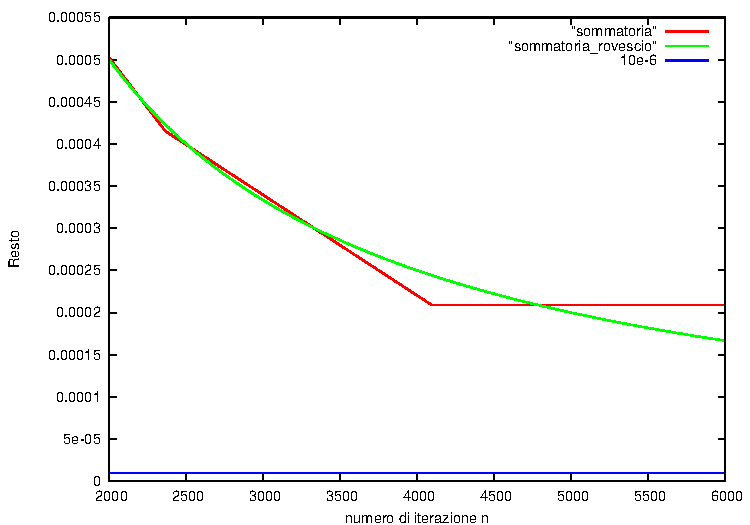
\includegraphics[width=14cm,keepaspectratio]{picture/confronto}
\caption{Confronto tra l'andamento del resto per il calcolo della serie con i due diversi algoritmi. In fondo è stampata anche la retta che indica l'incertezza legata all'allocazione come float}
\label{fig:confo}
\end{figure}

Come atteso, il risultato della sommatoria calcolata con il primo algoritmo raggiunge un limite di precisione. Il valore calcolato smette di migliorare quando il numero dell iterazioni supera la cifra $N =2^{p/2}$ iterazioni che nel caso del float ( p= 24 bit) corrisponde a $\sim 4000$.

Mentre il resto per la serie calcolata a rovescio continua a tendere a zero.
Fittando con la funzione $f(x) = A x^{B}$ l'andamento del resto calcolato con il secondo algoritmo si ottiene:

\begin{lstlisting}[frame=single]
After 22 iterations the fit converged.
variance of residuals (reduced chisquare) = WSSR/ndf   : 1.46634e-15

Final set of parameters            Asymptotic Standard Error
=======================            ==========================

B               = -0.999715        +/- 2.188e-06    (0.0002189%)
A               = 0.997602         +/- 1.669e-05    (0.001673%)
\end{lstlisting}

quindi un ottimo accordo con $ \textrm{resto} \sim \frac{1}{N}$.

Da ciò si può concludere che il miglior risultato (con minore incertezza) ottenibile si ha quando il resto è dell'ordine di grandezza dell'errore di allocazione del float $( \sim \pm 10^{-6} )$, ovvero troncando la serie ad  $N = 10^{6}$.

\begin{thebibliography}{99}
\bibitem{recipe}\emph{Numerical recipes in C++}
\bibitem{knuth}Knuth D. \emph{The Art of Computer Programming}
\bibitem{hilde}Hildebrand F. \emph{Introduction to Numerical Analysis}, 2nd.ed.
\end{thebibliography}
\end{document}
